\documentclass{beamer}

\usepackage[utf8]{inputenc}
\usecolortheme{beaver}
\usepackage{caption}
\usepackage{subcaption}
\usepackage{mathtools}
\usepackage{todonotes}
\usepackage{amsmath}
\usepackage{bm}
\usepackage{listings}
\usepackage{ragged2e}
\usepackage{fancyvrb}
\usepackage{titlecaps}

\Addlcwords{for a is but and with of in as the etc on to if}

\def\ci{\perp\!\!\!\!\!\perp}

\tikzstyle{latent} = [ draw, circle, inner sep = 2pt, minimum size = 0.65cm ]
\tikzstyle{observed} = [ draw, rectangle, inner sep = 2pt, minimum size = 0.65cm ]

\newtheorem{proposition}{Proposition}

\setbeamertemplate{section in toc}{\inserttocsectionnumber.~\inserttocsection}
\usetheme{Boadilla}
\makeatletter
\setbeamertemplate{footline}{%
    \leavevmode%
    \hbox{%
        \begin{beamercolorbox}[wd=.3\paperwidth,ht=2.25ex,dp=1ex,center]{author in head/foot}%
            \usebeamerfont{author in head/foot}\insertshortauthor\expandafter\beamer@ifempty\expandafter{\beamer@shortinstitute}{}{~~(\insertshortinstitute)}
        \end{beamercolorbox}%
        \begin{beamercolorbox}[wd=.55\paperwidth,ht=2.25ex,dp=1ex,center]{title in head/foot}%
            \usebeamerfont{title in head/foot}\insertshorttitle
        \end{beamercolorbox}%
        \begin{beamercolorbox}[wd=.15\paperwidth,ht=2.25ex,dp=1ex,right]{date in head/foot}%
            \usebeamerfont{date in head/foot}\insertshortdate{}\hspace*{2em}
            \insertframenumber{} / \inserttotalframenumber\hspace*{2ex} 
        \end{beamercolorbox}}%
        \vskip0pt%
    }
\makeatother

\begin{document}

\title[]{Validating Causal Inference Methods}
\author [] {}
\date{}

\begin{frame}
	\frametitle{Motivation}
	\begin{itemize}
		\item Many statistical methods for causal inference under unconfoundedness conditions. E.g. proposity score method, doubly robust, etc.
		\item These methods have only been evaluated on simualted data which might not be representative of real at hand.
		\item Crucial to understand how these methods perform on the data at hand.
	\end{itemize}
	\begin{figure}
		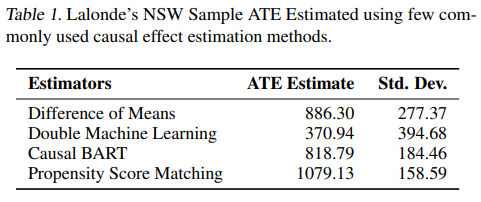
\includegraphics[scale=0.6]{imgs/comparison.png}
	\end{figure}
\end{frame}

\begin{frame}
	\frametitle{\titlecap{Proposed Framework}}
	\vspace{-2em}
	\begin{figure}
		\centering
		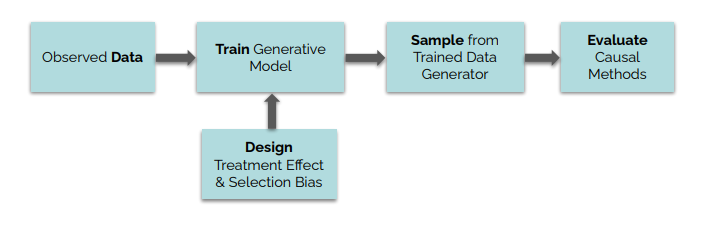
\includegraphics[scale=0.65]{imgs/flow.png}
	\end{figure}
	\vspace{-1.5em}
	\begin{itemize}
		\item A synthetic data generation approach.
		\item Uses user specified form and magnitude of causal effects
			and confounding bias.
		\item Trains a generative model that can generate
			stochastically indistinguishable dataset.
		\item Evaluate the causal methods by comparing their estimates
			with the simulated data estimates.
	\end{itemize}
\end{frame}

\begin{frame}
	\frametitle{\titlecap{Proposed Framework}}
	\begin{figure}
		\centering
		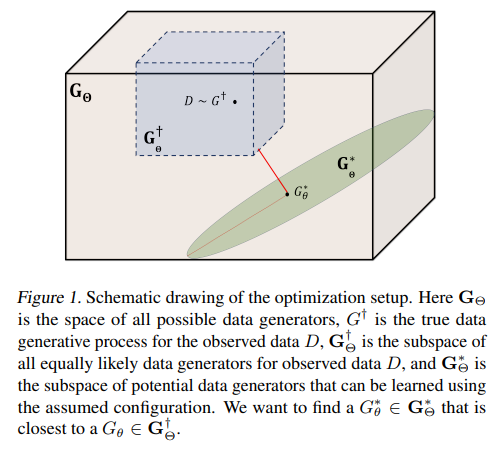
\includegraphics[scale=0.45]{imgs/distributions.png}
	\end{figure}
	\begin{itemize}
		\item Find a generative model such that:		
		\begin{equation*}
			\begin{split}
				min_{\theta} & \underbrace{\mathbb{E}[d((X, Y, Z), (X', Y', Z'))]}_{\text{Distribution dist.}} \\
				+ & \alpha \underbrace{\mid\mid \mathbb{E}[Y'(1) - Y'(0) \mid X'=x'] - f(x') \mid \mid}_{\text{Treatment effect error}}  \\
				+ & \beta \underbrace{\mid \mid \mathbb{E}[Y'(z') \mid X'=x', Z'=z'] - \mathbb{E}[Y'(z') \mid X'=x', Z'=1-z'] - g(x', z') \mid \mid}_{\text{confounding-bias error}} \\
			\end{split}
		\end{equation*}
	\end{itemize}
\end{frame}

\begin{frame}
	\frametitle{\titlecap{Proposed Framework}}
% 	\begin{tikzpicture}	
% 		\tikzstyle{every node}=[align=center, inner sep=1pt]
% 		\node (x) at (0, 0) {$ X $};
% 		\node (epsx) at (0, 1) {$ \epsilon_X $};
% 		\node (z) at (1, 0) {$ Z $};
% 		\node (epsz) at (1, 1) {$ \epsilon_Z $};
% 		\node (u) at (2, 1) {$ U $};
% 		\node (y) at (3, 0) {$ Y $};
% 		\node (epsy) at (3, 1) {$ \epsilon_Y $};
% 
% 		\draw [->] (epsx) -- (x);
% 		\draw [->] (x) -- (z);
% 		\draw [->] (epsz) -- (z);
% 		\draw [->] (u) -- (z);
% 		\draw [->] (epsy) -- (y);
% 		\draw [->] (z) -- (y);
% 		\draw [->] (u) -- (y);
% 	\end{tikzpicture}
	\begin{columns}
		\begin{column}{0.8 \textwidth}
	\begin{itemize}
		\item Trains two conditional VAEs for: 
			\begin{enumerate}
				\item $ P(X \mid Z) $: Loss function $ \sum_{i=1}^{N} \mid \mid X_i - X_i' \mid \mid_2 + D_{KL}(\mathcal{N}(\mu_i^X, \Sigma_i^X \mid \mid \mathcal{N}(0, 1)) $
				\item $ P(Y \mid X, Z) $: Loss function
					\begin{equation*}
						\begin{split}
							\frac{1}{N} & \sum_{i=1}^{N} \mid \mid Y_i - (Z_i Y_i'(1) + (1 - Z_i)Y_i'(0)) \mid \mid_2  \\
							& + D_{KL}(\mathcal{N}(\mu_i^Y, \Sigma_i^Y) \mid \mid \mathcal{N}(0, 1)) \\
							& + \alpha \mid \mid Y_i'(1) - Y_i'(0) - f(X_i) \mid \mid \\
							& + \beta \mid \mid Y_i'(1-Z_i) - Y_i''(1-Z_i) - g(X_i, Z_i) \mid \mid
						\end{split}
					\end{equation*}
			\end{enumerate}
		\end{itemize}
		\end{column}
		\begin{column}{0.2\textwidth}
			\begin{figure}[t]
			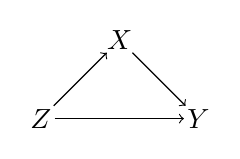
\begin{tikzpicture}	
			\tikzstyle{every node}=[align=center, inner sep=1pt]
				\node (z) at (0, 0) {$Z$};
				\node (x) at (1, 1) {$X$};
				\node (y) at (2, 0) {$Y$};

				\draw[->] (z) -- (x);
				\draw[->] (x) -- (y);
				\draw[->] (z) -- (y);
			\end{tikzpicture}
			\end{figure}
		\end{column}
	\end{columns}
	\begin{itemize}
		\item Use these VAEs to simulate data: $ (X', Z', Y'(1), Y'(0)) $ with known treatment effect.
		\item Compare it with treatment effect estimated by causal inference methods.
	\end{itemize}
\end{frame}

\begin{frame}
	\frametitle{\titlecap{Discussion Points}}
	\begin{itemize}
		\item Multiple causal models can generate the same
			observational dataset. How realistic is the assumption
			that the causal effect estimate from the generative
			model is same as the true DGP.
		\item Why is specifying the treatment effect and confounding
			bias a desirable propoerty?
		\item What is the data that the VAE is getting trained on? What
			did they mean by training it on a set of global
			datasets?
		\item Extending the approach for estimating other metrics like
			Conditional ATE?
		\item Can a single VAE be trained?
	\end{itemize}
\end{frame}
\end{document}
